% arara: pdflatex

\documentclass[tikz,border=0pt]{standalone}
\usepackage{pgfplots}
\usepackage{xcolor}
\usepackage{siunitx}

\usetikzlibrary{arrows}

% original colors
\definecolor{color1}{RGB}{166,118,29}
\definecolor{color2}{RGB}{217,95,2}
\definecolor{color3}{RGB}{231,41,138}
\definecolor{color4}{RGB}{117,112,179}
\definecolor{color5}{RGB}{27,158,119}
\definecolor{color6}{RGB}{102,166,30}
\definecolor{color7}{RGB}{230,171,2}

\definecolor{amber(sae/ece)}{rgb}{1.0, 0.49, 0.0}

\begin{document}
\begin{tikzpicture}
% \clip (-5.59cm, -3.6cm) rectangle (5.59cm, 3.49cm);
\newcommand{\figwidth}{8.64cm}
\newcommand{\figheight}{3.52cm} % golden ratio
\draw[use as bounding box, white] (0,0) rectangle (\figwidth,\figheight);

\node[inner sep=0pt, anchor=south west] (image) at (0,0)
{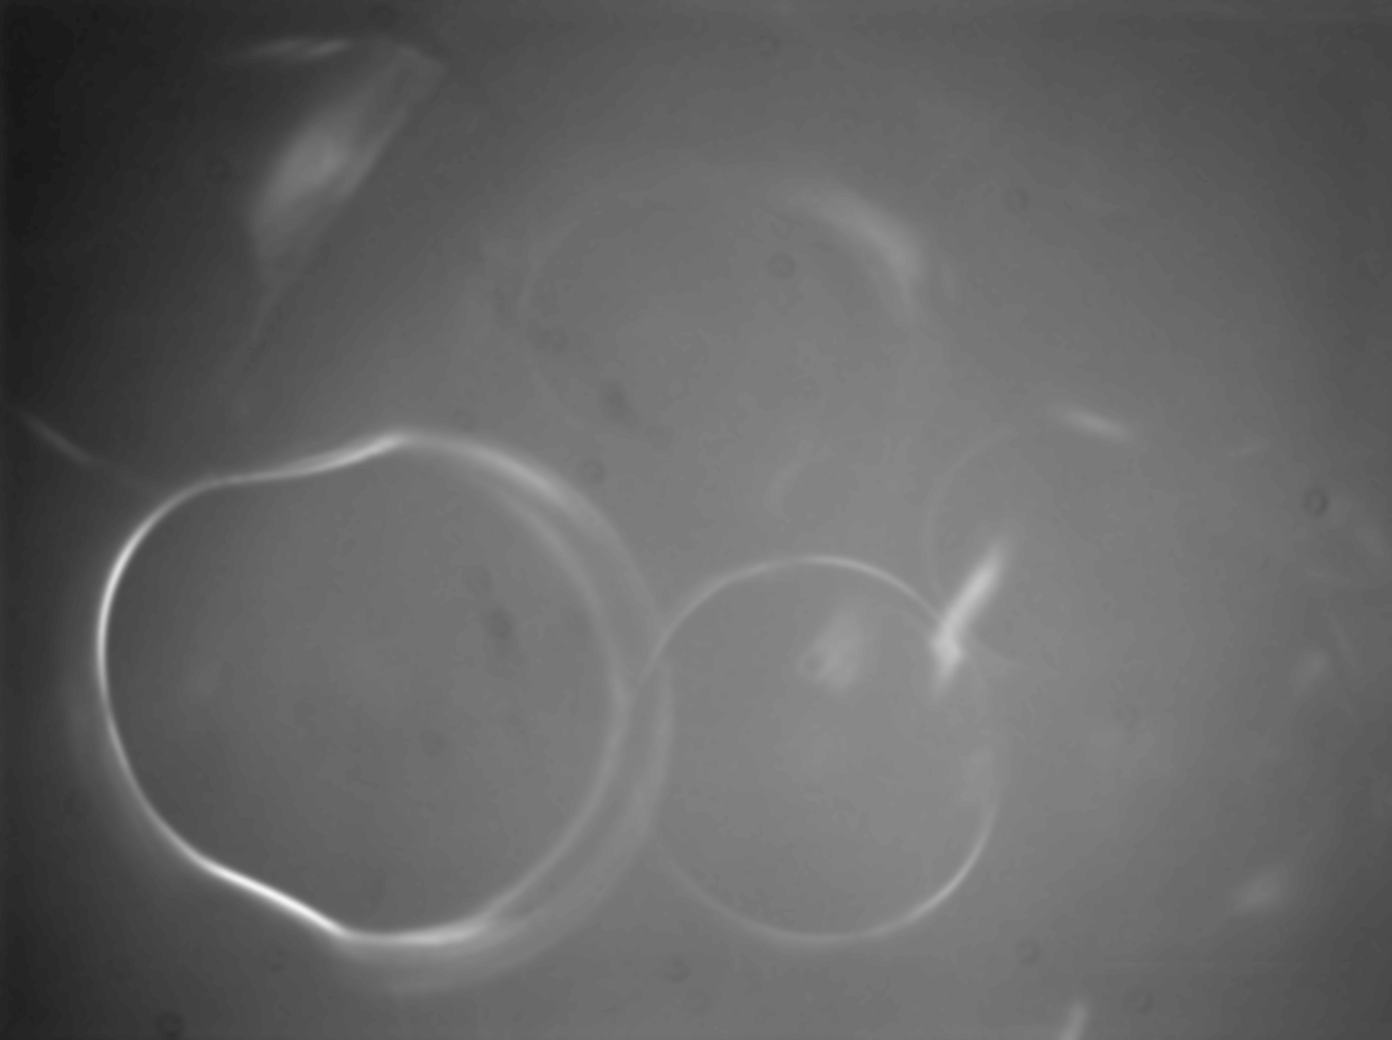
\includegraphics[width=4.3cm,height=3.5cm,
                  trim={0.0cm, 0cm, 0.0cm, 0cm}, 
]{waterinoil2.png}};

\node[inner sep=0pt, anchor=south east] (image) at (\figwidth,0)
{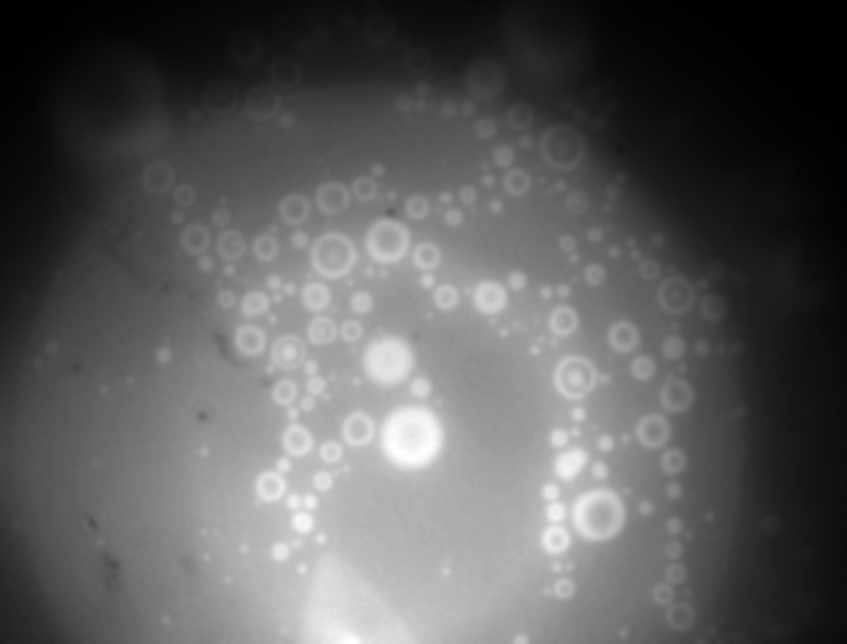
\includegraphics[width=4.3cm,height=3.5cm,
                  trim={0.0cm, 0cm, 0.0cm, 0cm}, 
]{oilinwater2.png}};

% scale bar left
\begin{scope}[
    xshift=3.05cm,
    yshift=2.85cm,
]
   \fill[fill=white, fill opacity=0.25] (0.0mm, 0.0mm) rectangle ++(12mm, 6.0mm);
   \draw [white, line width=0.3em] (1.25mm, 4.7mm) --
       node[below=0.3mm,inner sep=0.1em, font=\normalsize] {\SI{100}{\micro\metre}}
       ++(9.57mm, 0mm);
\end{scope}

% scale bar right
\begin{scope}[
    xshift=7.37cm,
    yshift=2.85cm,
]
   \fill[fill=white, fill opacity=0.25] (0.0mm, 0.0mm) rectangle ++(12mm, 6.0mm);
   \draw [white, line width=0.3em] (5.4mm, 4.7mm) --
       node[below=0.3mm,inner sep=0.1em, font=\normalsize] {\SI{10}{\micro\metre}}
       ++(1.57mm, 0mm);
\end{scope}

%\begin{scope}[
%    xshift=-0.3cm,
%    yshift=2.9cm,
%    ->,
%    >=stealth',
%    very thick,
%]
%  \node at (-3cm,0) (1) {};
%  \node at (3cm,0) (2) {};
%  %\path[white] (2) edge[bend left=10] node [above] {\huge$\omega_i$} (1);
%  \path[white] (2) edge[bend left=10] node [above] {\Large Inner cylinder} (1);

%\end{scope}

% labels
\node[white] at (0.22cm, 3.30cm) {\textbf{A}};
\node[white] at (4.55cm, 3.30cm) {\textbf{B}};

\end{tikzpicture} 
\end{document}
